\documentclass[journal]{IEEEtran/IEEEtran}

\usepackage[utf8x]{inputenc}
\usepackage{cite}
\usepackage{hyperref}
\usepackage{url}
\usepackage{verbatim}
\usepackage{epstopdf}
\usepackage{amssymb}
\usepackage[pdftex]{graphicx}
\graphicspath{{img/}}
\DeclareGraphicsExtensions{.eps,.pdf,.png,.jpg,.jpeg}
\usepackage[cmex10]{amsmath}
\usepackage{array}

\usepackage{fancyvrb}
\DefineVerbatimEnvironment{code}{Verbatim}{fontsize=\small}


% correct bad hyphenation here
\hyphenation{op-tical net-works semi-conduc-tor}

\begin{document}
\title{Data Stream Analisys and Data Mining With Storm}

\author{Gregor~Majcen, Miha~Zidar}%
\markboth{MLDM Workshop, January~2013}{}
%\IEEEspecialpapernotice{(Invited Paper)}
\maketitle
\begin{abstract}
    Twitter Storm is a powerfull distributed real-time data processing solution, with a wide range of usage. In this paper, we are going to take a look at how we can utilize Twitter Storms power for data mining on streams of data. The main focus of this paper is real-time data processing and online data mining.
\end{abstract}

\begin{IEEEkeywords}
    online learning, continuous data, data mining, distributed systems, horizontal scaling, batch processing
\end{IEEEkeywords}

\IEEEpeerreviewmaketitle


\section{Introduction}
\IEEEPARstart{T}{oday} we are generating more data per second than ever before, and the amount of data produced is only increasing over time. Data on its own is not that useful for us, unless we can extract information from it and the speed of gathering that information is becomming more and more valuable. This is where the real-time data processing comes in. Big companies like Twitter, Groupon, spider.io and others, are using Twitter Storm to provide a better user experience.\\

In the last few years data processing has come a long way with services like MapReduce, Amazon EMR, Hadoop, and related techologies. All of these were made to handle massive amounts of data, and they do that very affectively. But lately their weakness is showing in their lack of real-time processing. Now speed is starting to be ever more important, to get ahead of competition. This is where Storm comes in. Unlike other solutions that work in "batch" mode, Storm is made so it can handle data streams. With that it's possible to get calculations done on tupples of data and have the results back in matter of seconds, insted of hours or even days. One valuable ability to have, with ever increasing data streams, is scalability. To be more precise, horizontal scalability, where if the data stream grows, we can simply add more nodes withought having to increase the speed of each individual node, and Twitter Storm prodvides that by running on top of Apache Zookeeper cluster.

Handling large data streams has always been possible even without Storm, but that meant handling queues and workers and dispatchers. Usually those present a problem with scaling, since dispatchers have to be modified to support new queues for the new workers. Thus a lot of the work with such system is just to keep the system running, insted of actually working on the logic of the workers. Storm keeps our focus on the actual logic of the topology, and it hadles the queues and dispatchers so we do not have to. \\

We will begin by explaining what Storm is, how it works, and what it is used for. Then we shall slowly narow down all the Storm uses to the ones that become useful in datamining. We will show a simple storm demo project, and discuss how these concepts can be applied to machine learning. At the end we will look at a practical machine learning algorithm running on Storm, then we'll take that knowlage to hypothesise a solution for the stock market prediction.

%\hfill mds%?
%\hfill \today

\section{Twitter Storm}
Storm is an open source distributed and fault-tolerant real-time computation system, that is writen in clojure and runs on JVM. It provides a high abstraction layer with witch we can run complex computations on a cluster of computers. Storm provides users with a general framework for performing computataions on data streams in real-time, similar to how Hadoop provides users with a framework for performing batch processing operations. Because it runs on top of Zookeeper and has a good messageing system using tupples of data, it provides a good alternative to managing your own cluster with queues and workes. \\

Storm can be used for stream processing, processing messages, updating databases, updating online machine learning models in real-time. Other uses also include continuous computation, doing a continuous query on data streams and streaming out the results to users as they are computed, and for distributed RPC. 


\subsection{Storm structure}
Befor we can start anything, we need to learn Storms terminology. Even though Storm is oftene refered as Hadoop in real-time, the fact that it handles data streams and does not by it self store data or even finishes proceesing, means that it can not be compared to it or any other batch method. That is why storm does not have processes, but it calls those topologies, which unlike a process never finish.\\

The two main parts of topologies are sprouts and bolts. Each spout and bolt runs in multiple instances called taskes \ref{tasks}, that are distributed on a storm cluster \ref{stormcluster}. The number of task given to a bolt is determened in our program and is does not depend on the underlying structure of the Storm cluster. That makes adding and removing nodes from the cluster easy and requires no extra programming work. Another useful feature of Storm is that both spots and bolts can be writen in any more popular programming language, as long as the code provides a simple API that the storm can use for comunication. \\

\begin{itemize}
    \item \textbf{spout} - this is basically the input for the entire system, it is the point (or multiple points) where the outside data streams are connected. The main task is to fetch data and convert it to tuples so that bolts can access it. For example, spout could read from a Kestrel queue, Twitter streaming API, directly read some sensor, or it could even scrape data from the web.\\
    \item \textbf{bolt} - a simple operating unit, that recieves and processes data from sprouts or bolts and possibly generates an output stream for other bolts. Bolts can be simple functions that modify, filter, aggregate or join data, or talk to databases. \\
    \item \textbf{stream} - unbound sequence of tuples that is created and processed in a parallel using a distributed cluster. Streams are used to connect spouts and bolts. Since spouts and bolts run in multiple tasks, \textit{Stream Grouping} defines how a stream is being partitioned between those tasks. Storm supports four types of stream groupings:
        \begin{itemize}
            \item \textit{Shuffle grouping} - picks a random task, 
            \item \textit{Fields grouping} - mod hashing on a subset of tuple fields, 
            \item \textit{All grouping} - send to all tasks, 
            \item \textit{Global grouping} - pick task with lowest id
        \end{itemize} 
        \ \\
    \item \textbf{topology} - a complete Storm structor similar to a never ending process. It is composed of spouts and bolts which are connected with data streams between them. \ref{topology} \\
\end{itemize} 
\ \\

Storm topologies run on top of Storm cluster \ref{stormcluster}. A Storm cluster is made up of two kinds of nodes: the master node and the worker nodes. The master node runs a daemon called \textit{Nimbus} which distributes the code to worker nodes around the cluster, assignes tasks to individual machines and monitors to faliures. Every worker node runs a daemon called \textit{Supervisor} that listens for work assigned to it by Nimbus and starts or stops worker processes to do the assigned task. The coordination between Nimbus and Supervisors is done through a Zookeeper cluster.


\begin{figure}[htbp]
    \begin{center}
        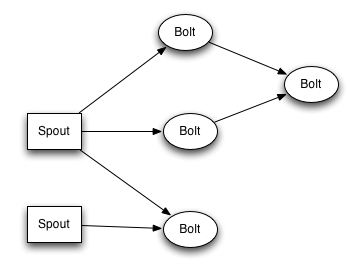
\includegraphics[scale=0.55]{img/topology.png}
        \caption{Storm topology structor}
        \label{topology}
    \end{center}
\end{figure}

\begin{figure}[htbp]
    \begin{center}
        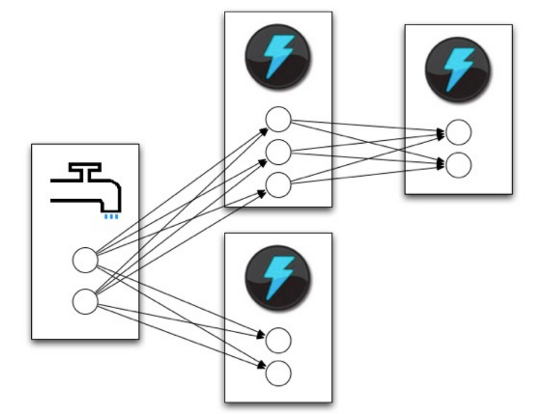
\includegraphics[scale=0.40]{img/tasks.png}
        \caption{Spouts and Bolts running as task and connected with streams.}
        \label{tasks}
    \end{center}
\end{figure}

\begin{figure}[htbp]
    \begin{center}
        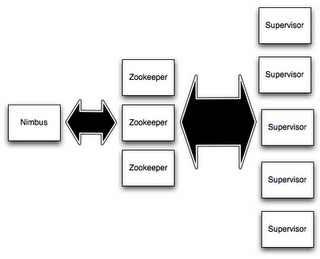
\includegraphics[scale=0.70]{img/storm-cluster.png}
        \caption{Storm cluster}
        \label{stormcluster}
    \end{center}
\end{figure}


\subsection{Usage}

There are three basic ways, how Storm can be used, depending on our needs. \\

\begin{itemize}
    \item \textbf{Stream processing} - processing a stream of new data and updating databases in real-time. Unlike the standard approach of doing stream processing with queues and workers, Storm is fault-tolerant and easily scalable. A use case for data mining would be to have an online learner that we would continously update, so it would always take into considuration the latest data points we have. Since Storm is falut-tolerant, this would mean that we would not loose any knowledge.\\
    \item \textbf{Distributed RPC} - computing an intense query on the fly in parallel. With distributed RPC, a Storm topology is a distributed function that you can invoke like a normal function. This could be used to build bigger ensamble models, in a paralell fashion. Another use case would be to classify a data point with a big ensable model, where each classifier would run as an indiptendent task.\\
    \item \textbf{Continous computation} - streaming the results of a query to clients to visualize in real-time. An example is streaming trending topics on Twitter into browsers. A use case for this would be if we have a model that can be improved with time, such as a large neural network, or running genetic algorithms.\\
\end{itemize}


\subsection{Simple Example}

Main class that defines how spouts and bolts are connected.

\begin{code}
     
    builder = new TopologyBuilder();

    builder.setSpout(
        "spoutName",
        new SpoutClass(args),
        10 // number of tasks
    );

    builder.setBolt(
        "boltName",
        new BoltClass(args),
        15 // number of tasks
    ).shuffleGrouping("spoutName")

\end{code}

Simple spout example that just generates random strings. In real world example, this spout would contain the code to read input streams, such as twitter API.

\begin{code}

public class SpoutClass extends BaseRichSpout {
    SpoutOutputCollector collector;

    // override open method and set collector

    @Override
    public void nextTuple() {
        // result should read real data from
        // outside world
        Values res = new Values("Hello World");
        collector.emit(res);
    }

    // override ack and fail methods

    @Override
    public void declareOutputFields(
            OutputFieldsDeclarer declarer) {
        declarer.declare(new Fields("word"));
    }
    
}

\end{code}

Simple bolt that just splits a sentence into individual words. The main class is written in java, but the logic is implemented in python. 

\begin{code}

public static class BoltClass 
        extends ShellBolt 
        implements IRichBolt {
    
    public SplitSentence() {
        super("python", "splitsentence.py");
    }

    public void declareOutputFields(
            OutputFieldsDeclarer declarer) {
        declarer.declare(new Fields("word"));
    }
}

\end{code}

The python code for our word splitting bolt.

\begin{code}

import storm
class BoltClass(storm.BasicBolt):
    def process(self, tup):
        words = tup.values[0].split(" ")
        for w in words:
            storm.emit([w])

\end{code}


\subsection{Possible applications of Storm}


\begin{itemize}
    \item \textbf{preprocessing} - Storm topologies can be used for machine learning indirectly, just for data preprocessing before running the data on a machine learning algorithem. The most common use for this would be video analizing, image streams such as tumblr, or any other data type that needs preprocessing before any classification or regression algorithms can be run.\\

    \item \textbf{prediction} - For this use case, Storm could be used as a distributed RPC that would classify each instance from a given fixed ensamble model. Here different bolts would perform their classification based on different models and some bolts would take care of stacking. The benifit of using storm here is that it would be trivial to scale such a system to best fit the current demand. 
\\
    \item \textbf{learning} - Used with MOA or any other framework, Storm could help with the learning of online algorithms. The learning bolts would spawn many tasks, to acomodate a stream that would normally be too large for a single machine to handle.\\
\end{itemize}


\section{Online machine learning}

Online machine learning, is an induction model for learning from one instance at a time. This makes online algorithems perfect for data streams, since the model can be easily and constantly adjusted to acomodate for the newer data. As long as a good clasifier exists, the online algorithem will eventually learn to make better predictions. Online algorithems work with a sequence of trials, each of those can be represented with three steps. In the first step, the algorithm receives an instance, then in the second step, it predicts the label of the instance, and in the last step the algorithm receives the true label of the instance. The third step then also corrects the hypothesis to minimize the error, hopefully to make better predictions for future trials. \\

One drawback of these algorithems, is the need for more and more correctly labeled examples from which the algorithem would learn. This ofcourse is not possible, when correctly labeling an example costs money and time. Fortunately there are a lot of problems where the correct label is always available. For example any problem that has to do with predicting the future. In those problems the label will eventually be available and the algorithem will be able adjust its model to compensate the new data. A case of a future prediction problem would be movements on the stock market, or finding the next trending topic on twitter. \\

A few popular online machine learning algorithems are:\\
\begin{itemize}
    \item \textit{perceptoron} - algorithm for supervised classification of an input into one of seven possible non-binary outputs. The learning algorithm for perceptrons is an online algorithm, which means that it can processes elements in the training set one at a time.\\
    \item \textit{LASVM} - relies on the traditional “soft margin” SVM formulation, handles noisy data sets, and is nicely related to the SMO algorithm. Experimental evidence on multiple data sets indicates that it reliably reaches competitive test error rates after performing a single pass over the training set.\\
    \item \textit{winnow} - algorithm for leraning a linear classifier from labeled examples, simmilar to perceptron. The algorithm can be used in the online learning setting, where the learning and the classification phase are not clearly separated.\\
    \item \textit{naive bayes} - the bayesian online algorithm is a method for estimating parameters using the power of bayesian inference.\\
    \item \textit{naive bayes multinomial} - simmilar to naive bayes, except that the probability distribution is multinomial, which is good for data that can be turned into counts such as word counts and text.
\end{itemize}



\subsection{MOA - Massive Online Analysis}

MOA is an open source framework for data stream mining. It includes a collection of machine learning algorithms for classification, regression, and clustering and tools for evaluation. MOA is related to the WEKA project and is also written in Java. MOA can perform data stream mining in real time. MOA can be easily used with Hadoop, S4 or Storm, and extended with new mining algorithms, and new stream generators or evaluation. A normal data mining approach may allow larger data sets to be handled, but it lacks the ability to process a continuous supply of data. The data stream paradigm has recently emerged in response to the continuous data problem. Algorithms written for data streams can naturally cope with data sizes many times greater than memory, and can extend to challenging real-time applications not previously tackled by machine learning or data mining.

\section{Simple example with Storm, Moa and Weka}

As we have seen in the previous sections, Storm is a very powerful tool, used for a lot of different purposes. In this section, we will see implications Storm has in the data mining field. For this we will examine a simple project that tries to classify reddit posts into specific subreddits. The following project serves only as an example, and at the end of this section, we will discuss how these principles can be applied to real world problems.

\subsection{Explanation of the algorithm}

This storm topology, spouts fetch posts from a few subredits and hand them over to classifier bolts. The classifier bolt then takes each touple, which reprisents one learning instance, and trys to correctly classify in which subredit it belongs, and then it updates the classifier with the training instance. In a real world, if we were for example predicting how many upvotes a post will get in the first hour, the delay between the classification and updating the classifier would be bigger. Because of this, we chose a problem, where we would not have to wait as long for updating the classifier. 

\subsection{Spout}

Reads the imput stream from reddit API. To runn a spout, we provide the information on what subreddits we want to monitor. After the spout has been staretd, it fetches a short history of the posts in each subreddit and then waits for the next post. Because reddit has caching and we can not get each new post as it comes, spouts look like they're gathering data in batches, but it is just a side effect of data selection, reddit API.

\subsection{Bolts}

The example contains four basic types of bolts; preprocessing bolt, classifier and learner, statistics printer, and statistics writer. All of these are connected in a linear fashion. \\

\begin{itemize}
    \item preprocessing - turnes the fetched reddit post into a word vector.\\
    \item classifier and learner - for this example we have used naive bayes, naive bayes multinomial and perceptron. they all have simmilar bolts and they all do the same, just with different classifiers. So all the bolts first get a single data instance in form of a tuple containg a word vector and the correct classification class. Then that word vector gets classified with either of the previos three classifiers and then the model gets trained on that data with the correct class. The output tuple from these bolts contains the predicted and the correct class. \\
    \item statistics printer - calculates the classification accuracy for each classifier and prints it on the screen if storm is running in local or debug mode.\\
    \item statistics writer - stores the data from the printer to a file. \\
\end{itemize}


\subsection{Results}

These are the results from our simple experiment, with a few thousand reddit posts and paralelism for each learner of 15 tasks, the results show how oniline algorithms can work with storm. To test the online classifiers working with the data stream, we tried running the test on 3 subreddits and on several. It is visible here that perceptron works nicely if the number of classes is low, and failes badly with a higer number of classes. The multinomial bayes performs well on all of the tests. Since this is just a proof oc concept, we did not run it on a data stream large enough to trully test the paralelism offered by Storm framework. This should be done and tested in the future.



\begin{figure}[htbp]
    \begin{center}
        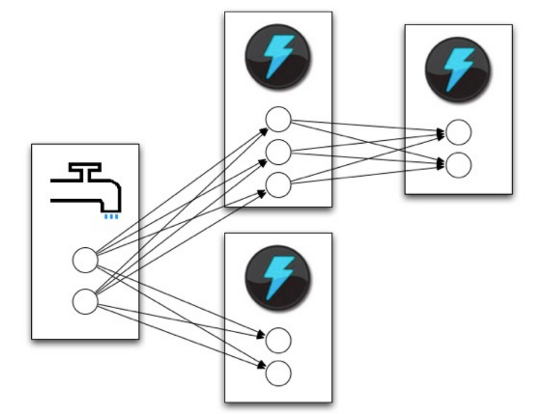
\includegraphics[scale=0.40]{img/tasks.png}
        \caption{Spouts and Bolts running as task and connected with streams.}
        \label{tasks}
    \end{center}
\end{figure}

\begin{figure}[htbp]
    \begin{center}
        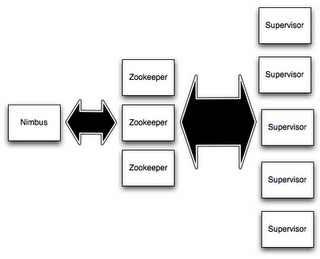
\includegraphics[scale=0.70]{img/storm-cluster.png}
        \caption{Storm cluster}
        \label{stormcluster}
    \end{center}
\end{figure}







\section{Conclusion}

Storm is a powerful and easy to use framework that can help us distribute the load for analysing a data stream, through our cluster. The hard part remains how to mold a problem in such a way that it can be scaled. If we are to write a simple learner and classifier and have Strom distribute that over 50 nodes, we would just get 50 different models and each case would get classified by just one of those. The prediction by the models could easily be stacked at some later point. If we try to have just one single model that learnes on different tasks running on different nodes, then we would have to do some extra work, since Storm does not have methods to syncronize the same class running on differen tasks. 

If we get our problem separated into different parts, then we are able to harness the full power of Storm, since it can efficiently process all the data. Storm had been benchmarked at processing one million 100 byte messages per second per node on a double Intel processor running at 2.4gh and with 24GB of memory. 


\appendices

\section*{Acknowledgement}
The authors would like to thank Matjaž Kukar, PhD Assistant Professor.


\begin{thebibliography}{1}
\bibitem{lasvm} Antoine Bordes, Seyda Ertekin, Jason Weston, Leon Bottou \emph{Fast Kernel Classifiers with Online and Active Learning} \relax 2005.
\bibitem{ibm} M. Tim Jones \emph{Process real-time big data with Twitter Storm} \relax 2012.
\bibitem{storm} Vaibhav Khadilkar, Murat Kantarcioglu, Bhavani Thuraisingham \emph{StormRider: Harnessing “Storm” for Social Networks} \relax .
\bibitem{ozaboost} Nikunj C. Oza, Stuart Russell \emph{Online Bagging and Boosting} \relax .
\bibitem{dmreview} Mohamed Medhat Gaber, Arkady Zaslavsky, Shonali Krishnaswamy \emph{Mining Data Streams: A Review} \relax .
\bibitem{moa} Albert Bifet, Geoff Holmes, Richard Kirkby, Bernhard Pfahringer \emph{Data Stream Mining, A partical approach } \relax 2011.
\bibitem{winnow} Nick Littlestone \emph{Learning Quickly When Irrelevant Attributes Abound: A New Linear-threshold Algorithm } \relax 1988.
\bibitem{bayes} Roberto C. Alamino, Nestor Caticha \emph{Bayesian online algorithms for learning in discrete hidden markov models} \relax 2006.
\bibitem{bayesmit} Manfred Opper \emph{A bayesian approach to online learning} \relax 1998.
\bibitem{tag} aut \emph{tiyyptle } \relax year.

\end{thebibliography}

\newpage

\begin{IEEEbiography}[{
\includegraphics[width=1in,height=1.25in,clip,keepaspectratio]{majcn}}]{Gregor Majcen}
63070199
\end{IEEEbiography}

% if you will not have a photo at all:
\begin{IEEEbiography}[{
\includegraphics[width=1in,height=1.25in,clip,keepaspectratio]{zidar}}]{Miha Zidar}
63060317
\end{IEEEbiography}
\end{document}


